\documentclass[12pt]{cornelltfpxsop}
\title{Cleanroom maintenance \newline}
%\date{August 6, 2015}
\date{\today}
\author{Jose Andres Monroy}
\approved{Jose Andres Monroy}
\sopid{CRM}
\sopversion{v1}
\sopabstract{This document describes the cleanroom and its regular maintenance.}

\begin{document}

\maketitle

%------------------------------------------------------------------
\section{Scope}
This document describes the maintenance of the cleanroom. It affects all persons using this room for any work in the scope of the project.

%------------------------------------------------------------------
\section{Purpose}
The cleanroom is a crucial part of the equipment to not only manufacture DEEs, but also for module testing and module-DEE integration. It provides a controlled environment for safe handling of modules and storage.

%------------------------------------------------------------------
\section{Definitions}

%------------------------------------------------------------------
\section{Responsibilities}
Every person is responsible to maintain a clean environment. While a minimum schedule for maintenance activities is outlined in this document, any person is allowed to trigger out-of-cycle maintenance if needed to maintain a clean environment.

%------------------------------------------------------------------
\section{Equipment}

\begin{itemize}
    \item Clean room
    \item Wipe pads, non-dusty tissues
    \item Swiffer ``Sweeper wet mop refills with Gain''
    \item Vacuum cleaner
    \item Sticky mats
\end{itemize}

% Consider adding images of key equipment if it helps

%------------------------------------------------------------------
\section{Procedure}

% Mention to record certain observations if this is needed
\subsection{Daily maintenance}
Needs to be done only if room in use. First person entering room is responsible and puts this on records.
\begin{enumerate}
    \item Inspect the cleanroom for any unusual dirt. If spotted, report and trigger a weekly maintenance.
    \item Check sticky mats. If excessive dirt is observed, change mats. Record this action.
    \item Clean your work space before starting to work and after you are done!  \textbf{remember: The standard is to leave no trace of your activity—or ideally, leave the workspace cleaner than you found it.}
\end{enumerate}

\subsection{Weekly maintenance}
\begin{enumerate}
    \item Inspect all tables and equipment surfaces (gantry, tables, coldbox, etc.). If dirt is visible, clean it using Isopropil-Alcohol (IPA) pads/wipes
    \item Clean floor using vacuum cleaner, followed by wet cleaning using Swiffer. 
        \begin{itemize}
            \item Follow the pattern as indicated in the figure \ref{moppath}, repeat the pattern every 30 sq/ft. Avoid circular motions
            \item Overlap paths to make sure no surface area is missed
            \item Mop in one direction
            \item Work backwards pulling the mop towards you
        \end{itemize}
    \begin{figure}
        \centering
        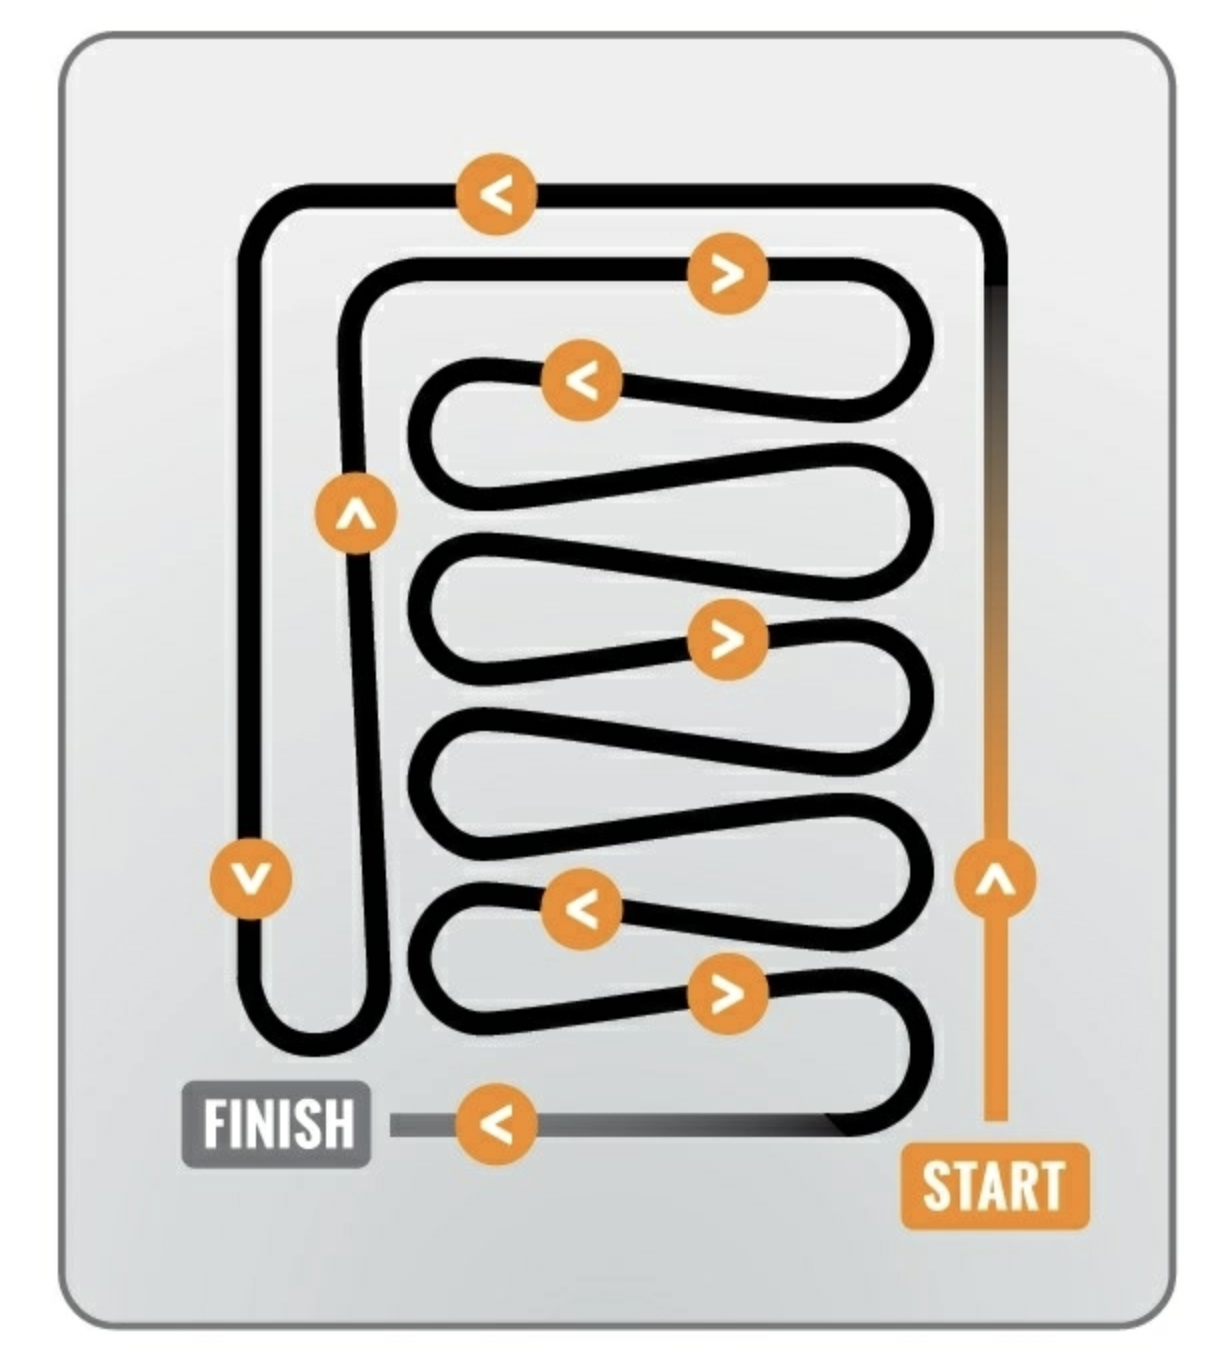
\includegraphics[width=0.8\linewidth]{img/moppath.jpg}
        \caption{mopping path}
        \label{moppath}
    \end{figure}
    \item Change sticky mats (inside and outside)
    \item Check gowning room. Remove unused items. Using Swiffer to clean floor (may reuse the tissue used inside cleanroom)
    \item Empty trash cans; dispose it appropriately
    \item Check for and report low supplies: gowns, booties, hair nets, gloves, IPA pads, lab books, etc.
    

\end{enumerate}

%------------------------------------------------------------------
\section{Documentation}
The following information must be recorded in the report for the Cornell E-log:\\ https://www.classe.cornell.edu/elog/TFPX/
\begin{itemize}
    \item Date, time (start--end) and operator name
    \item Any special observations, e.g.~damage to parts not already recorded during visual inspection, deviations from normal procedures
    \item Any action taken.
\end{itemize}

\end{document}


ISO 7 Cleanroom Cleaning Checklist & Guide
Daily Cleaning Checklist

[ ] Wipe work surfaces with 70% IPA
[ ] Clean equipment surfaces
[ ] Check and replenish cleaning supplies

Weekly Cleaning Checklist
[ ] HEPA vacuum floor
[ ] Clean behind/under fixed equipment
[ ] Inspect and clean overhead light fixtures
Entry Procedure
1. Enter the gowning area.
2. Remove external clothing.
3. Don gowning gear in this order: Shoe covers -> Hairnet -> Face mask -> Coverall -> Gloves.
4. Perform hand sanitization before entering the cleanroom.
5. Step onto the sticky mat before entry.
ISO 7 Cleanroom Cleaning Checklist & Guide
Cleaning Procedure Details
General Rules:
- Clean top to bottom, clean to dirty.
- Use straight, overlapping strokes (avoid circular motions).
- Change wipes, mops, and cleaning solution regularly.
- Use double-bucket system: one for detergent, one for rinsing.
- Always use cleanroom-approved cleaning agents and materials.
Floors:
- Vacuum first using HEPA-filtered vacuum.
- Mop with cleanroom detergent, using figure-eight motions.
- Final wipe-down with 70% IPA if required.
Equipment and Surfaces:
- Wipe down surfaces with 70% IPA daily.
- Clean high-touch points (handles, switches) multiple times per shift

